\chapter{Parallel Programming}\label{ch:b3:parallel-programming}

A laptop has many cores, and a program that uses one of them leaves the others idle. Splitting the \omterm{def:b3:parallel-programming:workspan}{work} is easy to start and hard to finish: the parts must not interfere, the time spent splitting and joining must stay small, and some steps cannot be split at all. This chapter measures what a split gains on the laptop, proves the two laws that bound it, models a computation as a graph whose total size and longest path decide how fast any number of processors can run it, and builds the parallel \omterm{def:b3:parallel-programming:scan}{prefix sum}, a small algorithm that looks sequential and is not. Along the way the Rust compiler refuses a data race, two threads slow each other down without sharing a single variable, and the C compiler turns one loop into instructions that add four numbers at once.

\begin{recall}
The threads of a process share its memory and run interleaved, in an order nobody controls; a data race is two unsynchronised accesses to one location by two threads, at least one a write. A cache keeps recently used memory in lines of 64 bytes close to the processor (Year~2 volume). Divide and conquer splits a problem into smaller ones of the same kind, and its cost satisfies a recurrence such as $T(n) = 2T(n/2) + n$, whose solution is $\Theta(n \log n)$ (Year~1 volume). A scoped thread in Rust may borrow from the function that spawned it, because the scope waits for it before returning.
\end{recall}

\section{Speed-up and its limits}\label{sec:b3:parallel-programming:speedup}

\begin{definition}[Speed-up, efficiency]\label{def:b3:parallel-programming:speedup}
Let $T_1$ be the time of a computation on one processor and $T_p$ its time on $p$ processors. Its \emph{speed-up}\index{speed-up} on $p$ processors is $S_p = T_1 / T_p$, and its \emph{efficiency}\index{efficiency (parallel)} is $E_p = S_p / p$. A speed-up of $p$, efficiency 1, is linear.
\end{definition}

The first program splits two jobs over $p$ scoped threads. One adds $2^{25}$ numbers, a job of one addition per number read from memory; the other runs a loop of shifts and exclusive ors on as many numbers, a job of 120 operations per number that touches no memory at all.

\omcode{code/bachelor-3/24-parallel-programming/listings/sum_threads.rs}{15}{42}{Each job cut into $p$ chunks, one scoped thread per chunk; the partial results are added after the threads are joined.}\label{lst:b3:parallel-programming:sum}

\omoutput{code/bachelor-3/24-parallel-programming/outputs/sum_threads.txt}{One run on the author's laptop, best of five for each $p$: the memory-bound sum stops near 3.5, the compute-bound loop reaches between 5 and 6.}\label{out:b3:parallel-programming:sum}

Neither job reaches 8. The compute-bound loop shares nothing, so its losses come from outside the program: the threads must be created and joined, and the laptop's cores also run other programs. The memory-bound sum stops earlier for a different reason, which no number of cores fixes: the cores share the path to memory, and a few of them already read as fast as it delivers.

Every program also has parts that do not split. If a fraction $f$ of its time on one processor is sequential, the rest gains at most $p$.

\begin{theorem}[Amdahl's law]\label{thm:b3:parallel-programming:amdahl}
If a fraction $f$ of a computation's time on one processor must run sequentially and the rest divides perfectly among $p$ processors, its \omterm{def:b3:parallel-programming:speedup}{speed-up} is $S_p = 1 / (f + (1 - f)/p)$, which increases with $p$ towards $1/f$ and never reaches it.
\end{theorem}

\begin{proof}
With $T_1 = 1$, the sequential part takes $f$ on any number of processors, and the rest takes $(1 - f)/p$, so $T_p = f + (1 - f)/p$ and $S_p = 1 / (f + (1 - f)/p)$. As $p$ grows the denominator decreases strictly towards $f > 0$, so $S_p$ increases strictly towards $1/f$ without reaching it.
\end{proof}

The law was presented by Gene Amdahl at a conference of 1967. % ledger: b3:amdahl-1967, b3:amdahl-named
Its lesson is severe: with 5\,\% of sequential \omterm{def:b3:parallel-programming:workspan}{work}, a million processors give less than 20.

\begin{omfigure}
\begin{tikzpicture}
  \begin{axis}[omrecord, width=0.72\linewidth, height=6cm, xlabel={processors $p$}, ylabel={speed-up $S_p$}, xmin=1, xmax=64, ymin=0, ymax=40, legend pos=outer north east, legend cell align=left, legend style={font=\small}, samples=64, domain=1:64]
    \addplot[black!40, dashed] {x};
    \addlegendentry{linear}
    \addplot[omDef, thick] {1/(0.01 + 0.99/x)};
    \addlegendentry{$f = 1\,\%$}
    \addplot[omDef, thick, dashed] {1/(0.05 + 0.95/x)};
    \addlegendentry{$f = 5\,\%$}
    \addplot[omThm, thick] {1/(0.1 + 0.9/x)};
    \addlegendentry{$f = 10\,\%$}
    \addplot[omThm, thick, dashed] {1/(0.2 + 0.8/x)};
    \addlegendentry{$f = 20\,\%$}
  \end{axis}
\end{tikzpicture}
\par\smallskip{\small Amdahl's law for four sequential fractions. With 1\,\% of sequential \omterm{def:b3:parallel-programming:workspan}{work}, 64 processors give 39; with 20\,\%, they give 4.7, and no number of processors gives 5.}
\end{omfigure}

Amdahl's law keeps the problem fixed. In practice a larger machine is used for a larger problem, whose parallel part grows while its sequential part stays the same, and the question becomes how much more \omterm{def:b3:parallel-programming:workspan}{work} fits in the same time.

\begin{theorem}[Gustafson's law]\label{thm:b3:parallel-programming:gustafson}
If a run on $p$ processors spends a fraction $f$ of its time in sequential \omterm{def:b3:parallel-programming:workspan}{work} and the rest with all $p$ processors busy, the same computation takes $f + (1 - f)p$ times longer on one processor: its scaled \omterm{def:b3:parallel-programming:speedup}{speed-up} is $p - f(p - 1)$.
\end{theorem}

\begin{proof}
Take the parallel run's time as 1. Its sequential part takes $f$ on one processor as well. Its parallel part keeps $p$ processors busy for $1 - f$, which is $(1 - f)p$ processor-time units, and one processor needs that long to do it. So $T_1 = f + (1 - f)p$ and $T_1 / T_p = f + (1 - f)p = p - f(p - 1)$.
\end{proof}

The law is named after John Gustafson and his colleague Edwin Barsis; Gustafson presented it in 1988 in an article titled \emph{Reevaluating Amdahl's law}. % ledger: b3:gustafson-1988, b3:gustafson-barsis
The two laws do not contradict each other: they answer different questions. With $f = 10\,\%$ measured on 8 processors, Gustafson's scaled \omterm{def:b3:parallel-programming:speedup}{speed-up} is 7.3, while Amdahl's law with $f = 10\,\%$ measured on one processor gives 4.7.

A \omterm{def:b3:parallel-programming:speedup}{speed-up} can even exceed $p$. When a job's data do not fit in one core's cache but its $p$ parts fit in $p$ caches, each part runs from its cache and the whole runs faster than $p$ times the original: the superlinear \omterm{def:b3:parallel-programming:speedup}{speed-up} comes from more cache, not from more processors.

\section{Task and data parallelism}\label{sec:b3:parallel-programming:kinds}

\begin{definition}[Task parallelism, data parallelism, fork--join]\label{def:b3:parallel-programming:kinds}
\emph{Data parallelism}\index{data parallelism} applies the same operation to different parts of the data at once, as the chunks of \cref{lst:b3:parallel-programming:sum}. \emph{Task parallelism}\index{task parallelism} runs different computations at once, such as the two recursive calls of a sort. In the \emph{fork--join}\index{fork--join} pattern, a computation forks into parts that run in parallel and continues only when all of them have finished, at the join.
\end{definition}

A recursive merge sort is \omterm{def:b3:parallel-programming:kinds}{fork--join}: the two halves are sorted in parallel, then merged. The C program below forks a thread at each of the top $\log_2 p$ levels of the recursion with POSIX threads, and joins it before the merge.

\omcode{code/bachelor-3/24-parallel-programming/listings/psort.c}{22}{40}{Fork the left half onto a new thread while this one sorts the right half; join, then merge.}\label{lst:b3:parallel-programming:psort}

\omoutput{code/bachelor-3/24-parallel-programming/outputs/psort.txt}{Sorting $2^{24}$ integers on the author's laptop, best of three: 4.5 with 8 threads.}\label{out:b3:parallel-programming:psort}

Each thread sorts its own range of the array, so no two threads write the same element. In C, nothing checks it. In Rust, the borrow checker does: a scoped thread may hold a mutable reference only if no other thread holds a reference to the same data, which is exactly the absence of data races.

\omcode{code/bachelor-3/24-parallel-programming/listings/race_reject.rs}{6}{21}{Two threads adding to one counter: a data race, written in Rust.}\label{lst:b3:parallel-programming:race}

\omoutput[1-21,29,31-32]{code/bachelor-3/24-parallel-programming/outputs/race_reject.txt}{The compiler's refusal, a staged error: the counter cannot be borrowed mutably by two threads at once. A note pointing into the standard library is left out.}\label{out:b3:parallel-programming:race}

The program is fixed by giving each thread its own counter and adding them after the join, as \code{sum_threads.rs} does, or by an atomic counter or a mutex; all three compile.

\section{Work and span}\label{sec:b3:parallel-programming:workspan}

A parallel program's running time depends on how many processors run it and how they are scheduled. Two numbers of the computation itself bound it whatever the machine.

\begin{definition}[Work, span, parallelism]\label{def:b3:parallel-programming:workspan}
A computation is modelled as a directed acyclic graph, its DAG: one node per operation, taking unit time, and an edge from each operation to every operation that uses its result. The \emph{work}\index{work (of a computation)} $W$ of the computation, also written $T_1$, is its number of nodes; its \emph{span}\index{span} $S$, also written $T_\infty$, is the number of nodes on a longest path, its critical path. Its \emph{parallelism}\index{parallelism (ratio)} is the ratio $W / S$.
\end{definition}

One processor runs one node per step, so it needs $W$ steps; infinitely many still need $S$, since the nodes of a path run one after the other. On $p$ processors, therefore, $T_p \ge W/p$ (the \omterm{def:b3:parallel-programming:workspan}{work} law) and $T_p \ge S$ (the \omterm{def:b3:parallel-programming:workspan}{span} law). The \omterm{def:b3:parallel-programming:workspan}{parallelism} is the largest \omterm{def:b3:parallel-programming:speedup}{speed-up} the computation allows: $T_1 / T_p \le W / S$.

\begin{omfigure}
\begin{tikzpicture}[font=\small, x=1.15cm, y=0.95cm, op/.style={draw, circle, minimum size=0.6cm, inner sep=0pt}, crit/.style={op, fill=omThm!25, very thick}]
  \node[crit] (a1) at (0,3) {1};
  \node[crit] (a2) at (0,2) {2};
  \node[op] (b1) at (2,3) {1};
  \node[op] (b2) at (2,2) {2};
  \foreach \k in {1,...,4} \node[crit] (c\k) at (1,2-\k) {\k};
  \draw[-{Stealth}, very thick, omThm] (a1) -- (a2);
  \draw[-{Stealth}] (b1) -- (b2);
  \draw[-{Stealth}, very thick, omThm] (a2) -- (c1);
  \draw[-{Stealth}] (b2) -- (c1);
  \foreach \k/\l in {1/2, 2/3, 3/4} \draw[-{Stealth}, very thick, omThm] (c\k) -- (c\l);
  \node[left=4pt of a1, align=right] {merge of\\ elements 0, 1};
  \node[right=4pt of b1, align=left] {merge of\\ elements 2, 3};
  \node[right=4pt of c2, align=left] {merge of the\\ two halves};
\end{tikzpicture}
\par\smallskip{\small The DAG of merge sort on four elements, each merge a chain of one step per element it outputs. \omterm{def:b3:parallel-programming:workspan}{Work} 8, \omterm{def:b3:parallel-programming:workspan}{span} 6; the shaded critical path runs through one of the two small merges, then the whole final merge.}
\end{omfigure}

The program below builds the DAGs of the chapter's algorithms node by node and measures them.

\omcode{code/bachelor-3/24-parallel-programming/listings/workspan.py}{8}{16}{\omterm{def:b3:parallel-programming:workspan}{Work} counts the nodes; \omterm{def:b3:parallel-programming:workspan}{span} is the largest depth, each node one deeper than its deepest input.}\label{lst:b3:parallel-programming:workspan}

\omoutput{code/bachelor-3/24-parallel-programming/outputs/workspan.txt}{\omterm{def:b3:parallel-programming:workspan}{Work}, \omterm{def:b3:parallel-programming:workspan}{span} and \omterm{def:b3:parallel-programming:workspan}{parallelism} of four DAGs. The merge sort's sequential merges cap its \omterm{def:b3:parallel-programming:workspan}{parallelism} at 5 for 1,024 elements.}\label{out:b3:parallel-programming:workspan}

A schedule decides which ready nodes run at each step; a node is ready when all its inputs have run.

\begin{definition}[Greedy scheduler, work stealing]\label{def:b3:parallel-programming:scheduler}
A \emph{greedy scheduler}\index{greedy scheduler} on $p$ processors never leaves a processor idle while a node is ready: at each step it runs $\min(p, r)$ of the $r$ ready nodes. Under \emph{work stealing}\index{work stealing}, each processor keeps a queue of the tasks it has forked and \omterm{def:b3:parallel-programming:workspan}{works} from it; a processor whose queue is empty takes a task from the queue of another, chosen at random.
\end{definition}

\begin{theorem}[Brent's theorem]\label{thm:b3:parallel-programming:brent}
A \omterm{def:b3:parallel-programming:scheduler}{greedy scheduler} runs a computation of \omterm{def:b3:parallel-programming:workspan}{work} $W$ and \omterm{def:b3:parallel-programming:workspan}{span} $S$ on $p$ processors in $T_p \le W/p + S$ steps. Since every schedule needs at least $\max(W/p, S)$ steps, a greedy schedule takes at most twice as long as the best one.
\end{theorem}

\begin{proof}
Call a step complete if it runs $p$ nodes, incomplete otherwise. Each complete step runs $p$ of the $W$ nodes, so there are at most $W/p$ complete steps. In an incomplete step, the \omterm{def:b3:parallel-programming:scheduler}{greedy scheduler} runs every ready node. Let $G$ be the DAG of the nodes not yet run; its sources are exactly the ready nodes, and every longest path of $G$ starts at a source, since a longest path that started below a node would extend to it. Running all the sources shortens every longest path of $G$ by its first node, so each incomplete step decreases the \omterm{def:b3:parallel-programming:workspan}{span} of $G$ by one, and there are at most $S$ of them. Hence $T_p \le W/p + S$. Every schedule takes at least $W/p$ steps and at least $S$ steps, so the best one takes $T^*_p \ge \max(W/p, S)$, and $W/p + S \le 2\max(W/p, S) \le 2T^*_p$.
\end{proof}

The theorem goes back to Richard Brent's paper of 1974 on evaluating arithmetic expressions in parallel. % ledger: b3:brent-1974, b3:brent-scheduling
The program below schedules two DAGs greedily and compares the result with both bounds.

\omcode{code/bachelor-3/24-parallel-programming/listings/brent.py}{12}{30}{A \omterm{def:b3:parallel-programming:scheduler}{greedy scheduler}: at each step it runs up to $p$ ready nodes, then counts down the inputs their users still wait for.}\label{lst:b3:parallel-programming:brent}

\omoutput{code/bachelor-3/24-parallel-programming/outputs/brent.txt}{A random DAG of 2,000 nodes and the merge sort of 256 elements, on 1 to 8 processors. Every time lies between the lower bound and Brent's bound; the worst ratio, 1.5, is the merge sort on 4 processors.}\label{out:b3:parallel-programming:brent}

On the random DAG, whose \omterm{def:b3:parallel-programming:workspan}{parallelism} is above 9, the greedy schedule is almost perfect for up to 8 processors. On the merge sort, \omterm{def:b3:parallel-programming:workspan}{parallelism} 4, the final merges leave processors idle, and adding them beyond 4 helps little. A real runtime does not see the DAG in advance: tasks appear as the program forks them. \omterm{def:b3:parallel-programming:scheduler}{Work stealing} balances them as they appear; Blumofe and Leiserson proved in 1999 that it runs a well-structured \omterm{def:b3:parallel-programming:kinds}{fork--join} computation in expected time $W/p + O(S)$, close to Brent's bound. % ledger: b3:blumofe-leiserson-1999

\section{Parallel algorithms}\label{sec:b3:parallel-programming:algorithms}

\begin{definition}[Parallel reduction, prefix sum]\label{def:b3:parallel-programming:scan}
A \emph{parallel reduction}\index{parallel reduction} combines $n$ values with an associative operation, such as $+$ or $\max$, by a tree of combinations: \omterm{def:b3:parallel-programming:workspan}{work} $n - 1$, \omterm{def:b3:parallel-programming:workspan}{span} $\lceil \log_2 n \rceil$. The \emph{prefix sum}\index{prefix sum}, or scan, of $a_0, \ldots, a_{n-1}$ is the sequence of running totals: inclusive, $a_0 + \cdots + a_i$ at position $i$, or exclusive, $a_0 + \cdots + a_{i-1}$, which starts with 0.
\end{definition}

Associativity is what allows the tree: $(a + b) + (c + d)$ equals $((a + b) + c) + d$, so the pairs can be added at the same time. Floating-point addition is not exactly associative, and a parallel sum of floats may differ in its last digits from the sequential one; the programs of this chapter add integers.

A scan looks sequential: each total needs the one before it. Hillis and Steele gave in 1986 a scan of \omterm{def:b3:parallel-programming:workspan}{span} $\log_2 n$, in which every element adds the one $2^d$ places to its left in round $d$; it does $n \log_2 n - (n - 1)$ additions instead of $n - 1$. % ledger: b3:hillis-steele-1986
Blelloch's scan does $2(n - 1)$, in a tree. % ledger: b3:blelloch-1989

\omcode{code/bachelor-3/24-parallel-programming/listings/scan.rs}{21}{52}{Blelloch's exclusive scan: the up-sweep leaves the sum of each subtree at its right end, the down-sweep hands each left subtree the total before it and each right subtree that total plus the left sum.}\label{lst:b3:parallel-programming:scan}

\omoutput{code/bachelor-3/24-parallel-programming/outputs/scan.txt}{The scan traced on eight days of rain, then the counted additions and rounds of both scans: Blelloch's does twice the minimum \omterm{def:b3:parallel-programming:workspan}{work}, Hillis and Steele's $\log_2 n$ times as much.}\label{out:b3:parallel-programming:scan}

\begin{omfigure}
\begin{tikzpicture}[font=\small, x=0.9cm, y=0.62cm, cell/.style={draw, minimum width=0.85cm, minimum height=0.55cm, inner sep=0pt}, new/.style={cell, fill=omDef!25}]
  \node[anchor=east] at (0.3,0) {rain};
  \foreach \v [count=\c] in {0,62,0,29,8,34,0,0} {
    \node[cell] at (\c,0) {\v};
  }
  \foreach \row/\name/\vals/\hot in {
      1/up 1/{0,62,0,29,8,42,0,0}/{2,6},
      2/up 2/{0,62,0,91,8,42,0,42}/{4,8},
      3/up 4/{0,62,0,91,8,42,0,133}/{8},
      4/down 4/{0,62,0,0,8,42,0,91}/{4,8},
      5/down 2/{0,0,0,62,8,91,0,133}/{2,4,6,8},
      6/down 1/{0,0,62,62,91,99,133,133}/{1,2,3,4,5,6,7,8}} {
    \node[anchor=east] at (0.3,-\row) {\name};
    \foreach \v [count=\c] in \vals {
      \node[cell] at (\c,-\row) {\v};
    }
    \foreach \h in \hot {
      \node[new] at (\h,-\row) {};
    }
    \foreach \v [count=\c] in \vals {
      \node at (\c,-\row) {\v};
    }
  }
\end{tikzpicture}
\par\smallskip{\small Blelloch's scan on the rain of eight days, in tenths of a millimetre, row by row as \code{scan.rs} prints it; shaded cells changed in that round. After the up-sweep the last cell holds the total, 133; it is replaced by 0 and the down-sweep ends with the exclusive running totals.}
\end{omfigure}

\begin{theorem}[Blelloch's scan]\label{thm:b3:parallel-programming:blelloch}
For $n = 2^k$, Blelloch's scan computes the exclusive \omterm{def:b3:parallel-programming:scan}{prefix sums} with $2(n - 1)$ additions in $2k$ rounds, the additions of each round being independent.
\end{theorem}

\begin{proof}
View positions $0, \ldots, n - 1$ as the leaves of a complete binary tree; a node of height $h$ covers $2^h$ consecutive positions and is stored at the last of them. \emph{Up-sweep.} In round $d = 2^{h-1}$, position $i$ adds position $i - d$: it then holds the sum of its node's left child (stored at $i - d$) and right child (stored at $i$), by induction on $h$. The positions written in one round are distinct and none is read by another addition of the round, so the additions are independent. Round $d$ does $n/(2d)$ additions, $n/2 + n/4 + \cdots + 1 = n - 1$ in all, in $k$ rounds. \emph{Down-sweep.} Claim: when the down-sweep reaches height $h$, the position of each node of height $h$ holds the sum of all positions before the node. It holds at the root, set to 0. At a node with that value $v$ stored at $i$, whose left child is stored at $i - d$ and still holds the left sum $\ell$ from the up-sweep, the round writes $v$ at $i - d$ and $v + \ell$ at $i$: exactly the sums before the left and the right child. At height 0 every position holds the sum before it. The down-sweep, too, does $n - 1$ independent additions in $k$ rounds.
\end{proof}

The DAG of \code{workspan.py} finds a \omterm{def:b3:parallel-programming:workspan}{span} of $2k - 1$, one less than the $2k$ rounds: the root's sum, computed by the last addition of the up-sweep, is replaced by 0, so no path runs through it into the down-sweep.

A scan on $p$ processors does not need a tree of $n$ leaves. The blocked scan of the weekend problem cuts the array into $p$ blocks: each processor sums its block, the $p$ sums are scanned, and each processor scans its block again from the total before it; exercise~\ref{exo:b3:parallel-programming:11} analyses it.

Parallel threads can also slow each other down without sharing data. A cache \omterm{def:b3:parallel-programming:workspan}{works} in lines of 64 bytes, and a core must hold a line on its own to write it; two cores writing two different variables of one line pass the line back and forth.

\begin{definition}[False sharing]\label{def:b3:parallel-programming:false-sharing}
\emph{False sharing}\index{false sharing} occurs when threads on different cores repeatedly write different variables that lie in the same cache line: the line moves between the cores' caches at every write, though no variable is shared.
\end{definition}

\omcode{code/bachelor-3/24-parallel-programming/listings/false_sharing.c}{11}{23}{Eight counters in one 64-byte line, or eight in eight lines; each thread adds to its own counter only.}\label{lst:b3:parallel-programming:false-sharing}

\omoutput{code/bachelor-3/24-parallel-programming/outputs/false_sharing.txt}{One run on the author's laptop, best of three: with 8 threads, the adjacent counters are about 17 times slower than the padded ones.}\label{out:b3:parallel-programming:false-sharing}

With one thread the two layouts take the same time. With 8, each thread does the same \omterm{def:b3:parallel-programming:workspan}{work} as alone, yet the adjacent counters take more than 30 times longer than with one thread, while the padded ones take less than twice as long. The fix is the padding of \code{struct padded}: one counter per line.

\section{Vector instructions and accelerators}\label{sec:b3:parallel-programming:simd}

\omterm{def:b3:parallel-programming:workspan}{Parallelism} also lives inside one core.

\begin{definition}[SIMD, vectorisation]\label{def:b3:parallel-programming:simd}
A \emph{SIMD}\index{SIMD} instruction (single instruction, multiple data) applies one operation to several values held side by side in a wide register, its lanes: a 16-byte register holds four 32-bit floats. \emph{Vectorisation}\index{vectorisation} is the compiler's rewriting of a loop so that each instruction processes several iterations, one per lane.
\end{definition}

A loop can be vectorised only if running several iterations at once gives the same result as running them in order. GCC reports what it did when asked.

\omcode{code/bachelor-3/24-parallel-programming/listings/saxpy.c}{1}{12}{Two loops over floats: each iteration of the first is independent, each iteration of the second needs the one before.}\label{lst:b3:parallel-programming:saxpy}

\omoutput{code/bachelor-3/24-parallel-programming/outputs/vec.txt}{The compiler vectorises the first loop with 16-byte vectors, and its remainder with 8-byte ones, but not the running sum. The assembly shows packed instructions (\code{ps}, four floats each) and scalar ones (\code{ss}, one float).}\label{out:b3:parallel-programming:vec}

The \code{restrict} qualifiers promise that \code{x} and \code{y} do not overlap; without them the compiler would have to check at run time that a write to \code{y} cannot change a later \code{x[i]}. The running sum is a scan, and its dependency of distance one keeps every lane waiting for the one before.

\begin{omfigure}
\raisebox{-0.5\height}{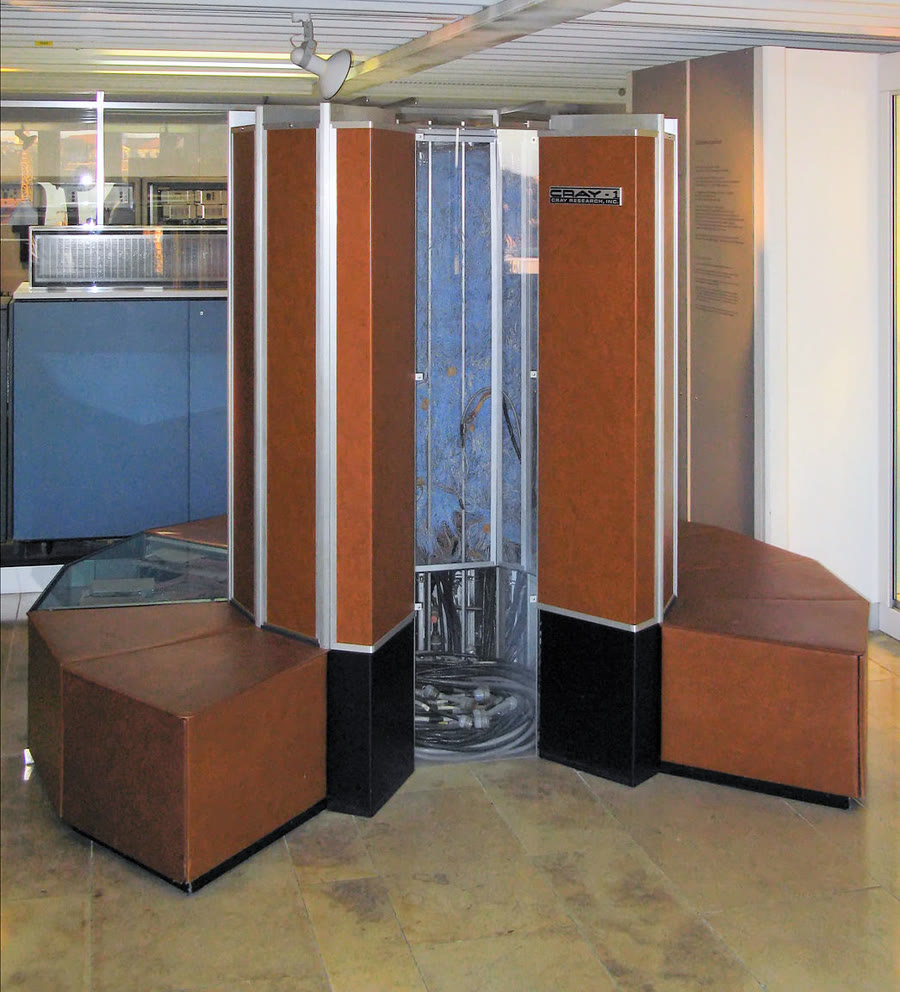
\includegraphics[width=0.42\linewidth]{images/book5/b3-24-cray-1.jpg}}\hfill
\begin{minipage}{0.52\linewidth}\small
A Cray-1 in the Deutsches Museum, Munich (photograph by Clemens Pfeiffer, 2006, CC BY 2.5). Designed by Seymour Cray and first installed at Los Alamos in 1976, it was the first supercomputer to implement the vector processor design successfully, at a peak of 160 million floating-point operations per second; eighty were sold. The benches around its base cover the power supplies. % ledger: b3:cray-1
\end{minipage}
\end{omfigure}

A graphics processor, or GPU, takes the same idea much further: thousands of lanes grouped into many cores, each group running one instruction on many data, with its own memory hierarchy between the lanes and the main memory. It suits \omterm{def:b3:parallel-programming:kinds}{data parallelism} on large arrays, the matrix products of neural networks above all; the One Artificial Intelligence Book and One Quant Book series return to it at length.

\section{Exercises}\label{sec:b3:parallel-programming:exercises}

\begin{exercise}[$\star$]\label{exo:b3:parallel-programming:1}
A program spends 10\,\% of its single-processor time in sequential \omterm{def:b3:parallel-programming:workspan}{work}. What \omterm{def:b3:parallel-programming:speedup}{speed-up} does Amdahl's law give on 8 processors, and what is its limit? What sequential fraction would allow a \omterm{def:b3:parallel-programming:speedup}{speed-up} of 6 on 8 processors?
\end{exercise}

\begin{exercise}[$\star$]\label{exo:b3:parallel-programming:2}
Draw the DAG of the evaluation of $(a + b)(c + d) + (e + f)(g + h)$, one node per operation. Give its \omterm{def:b3:parallel-programming:workspan}{work}, \omterm{def:b3:parallel-programming:workspan}{span} and \omterm{def:b3:parallel-programming:workspan}{parallelism}. Do the same for $((((a + b) + c) + d) + e)$.
\end{exercise}

\begin{exercise}[$\star$]\label{exo:b3:parallel-programming:3}
A computation has \omterm{def:b3:parallel-programming:workspan}{work} $10^6$ and \omterm{def:b3:parallel-programming:workspan}{span} $10^3$. Bound the time of a greedy schedule on 8 processors, and on 10,000, from above and below. Beyond how many processors can the \omterm{def:b3:parallel-programming:speedup}{speed-up} no longer grow much?
\end{exercise}

\begin{exercise}[$\star$]\label{exo:b3:parallel-programming:4}
\code{exercises/ex4_loops.c} holds three loops: \code{y[i] = 2 * y[i + 1]}, \code{y[i] = y[i - 4] + x[i]} and \code{y[i] = y[i - 1] + x[i]}. Predict which of them \code{gcc -O3} vectorises with 16-byte vectors of floats, then check with \code{-fopt-info-vec-optimized}.
\end{exercise}

\begin{exercise}[$\star\star$]\label{exo:b3:parallel-programming:5}
A parallel sum in C has each of its threads run \code{total += a[i]} on one global \code{total}. Run \code{exercises/ex5_interleave.py}, which plays the load, add and store of two threads in a scripted order, and explain the total it prints. Fix the C program so that it is correct for every interleaving without a lock in the loop.
\end{exercise}

\begin{exercise}[$\star\star$]\label{exo:b3:parallel-programming:6}
Write \texttt{par\_max(a:\ \&[i64], p:\ usize) -> Option<i64>}, which returns the largest element of \code{a} computed by $p$ scoped threads, and \code{None} if \code{a} is empty or $p = 0$. Test it against the sequential maximum.
\end{exercise}

\begin{exercise}[$\star\star$]\label{exo:b3:parallel-programming:7}
Prove that Hillis and Steele's scan is correct, does $n \log_2 n - (n - 1)$ additions for $n = 2^k$, and has \omterm{def:b3:parallel-programming:workspan}{span} $\log_2 n$. For $n = 2^{20}$ and 8 processors, compare the two scans by Brent's bound.
\end{exercise}

\begin{exercise}[$\star\star$]\label{exo:b3:parallel-programming:8}
Prove that the merge sort DAG of $n = 2^k$ elements, with sequential merges as in \code{workspan.py}, has \omterm{def:b3:parallel-programming:workspan}{work} $nk$ and \omterm{def:b3:parallel-programming:workspan}{span} $2n - 2$. What is its \omterm{def:b3:parallel-programming:workspan}{parallelism}, and why does the \omterm{def:b3:parallel-programming:workspan}{parallelism} of \code{psort.c} stay small?
\end{exercise}

\begin{exercise}[$\star\star$]\label{exo:b3:parallel-programming:9}
Starting threads has a cost: model the time on $p$ processors as $T(p) = f + (1 - f)/p + cp$, with $T_1 = 1$ apart from the cost. Find the real $p$ that minimises $T$, and the best integer $p$ and \omterm{def:b3:parallel-programming:speedup}{speed-up} for $f = 0.05$ and $c = 0.001$. What does the model say about adding processors beyond it?
\end{exercise}

\begin{exercise}[$\star\star\star$]\label{exo:b3:parallel-programming:10}
To merge two sorted arrays in parallel, take the median of the larger one, find by binary search where it falls in the other, and merge the two lower parts and the two upper parts in parallel. Prove that this merge has \omterm{def:b3:parallel-programming:workspan}{span} $O(\log^2 n)$ and \omterm{def:b3:parallel-programming:workspan}{work} $O(n)$, and deduce the \omterm{def:b3:parallel-programming:workspan}{work} and \omterm{def:b3:parallel-programming:workspan}{span} of the merge sort that uses it.
\end{exercise}

\begin{exercise}[$\star\star\star$]\label{exo:b3:parallel-programming:11}
Prove that the blocked scan of \cref{lst:b3:parallel-programming:weather} is correct for any $n$ and $p$. Count its additions, and its time on $p$ processors if each block costs its length and the middle scan is sequential. Show that its \omterm{def:b3:parallel-programming:speedup}{speed-up} over the sequential scan, counted in additions, stays below $p/2$, and say how to keep the middle step small for very large $p$.
\end{exercise}

\begin{exercise}[$\star\star\star$]\label{exo:b3:parallel-programming:12}
Model \code{psort.c}: below the top $\log_2 p$ levels each thread sorts $n/p$ elements alone, and at the top levels each merge is sequential. Derive $T_p$ and the \omterm{def:b3:parallel-programming:speedup}{speed-ups} the model predicts for $p = 2, 4, 8$ and $n = 2^{24}$, compare them with \cref{out:b3:parallel-programming:psort}, and explain the shape of the gap.
\end{exercise}

\section{Weekend problem}\label{sec:b3:parallel-programming:problem}

\begin{problem}[{Weekend problem --- Prefix sums of the town's weather}]\label{pb:b3:parallel-programming:1}
The town's two weather stations record the rain of every day. A running total answers questions such as how much rain fell between two dates: a subtraction of two totals. This problem computes the running totals of $2^{24}$ days, the town's two years repeated, sequentially and in parallel, and compares the parallel time with what the theory allows.

\omcode{code/bachelor-3/24-parallel-programming/listings/weather_scan.rs}{17}{42}{The blocked scan: each block summed by its own thread, the block sums scanned in order, each block scanned again from its offset.}\label{lst:b3:parallel-programming:weather}

\omoutput{code/bachelor-3/24-parallel-programming/outputs/weather_scan.txt}{One run on the author's laptop, best of five: the blocked scan against the sequential one, for 1 to 8 threads.}\label{out:b3:parallel-programming:weather}

\begin{omfigure}
\begin{tikzpicture}
  \begin{axis}[omrecord, width=0.72\linewidth, height=6cm, xlabel={threads $p$}, ylabel={speed-up}, xmin=1, xmax=8, ymin=0, ymax=8, legend pos=north west, legend cell align=left, legend style={font=\small}]
    \addplot[black!40, dashed, domain=1:8] {x};
    \addlegendentry{linear}
    \addplot[omDef, thick, mark=*] table[x=p, y=cpu] {code/bachelor-3/24-parallel-programming/figures/speedup.dat};
    \addlegendentry{compute-bound loop}
    \addplot[omDef, thick, dashed, mark=o] table[x=p, y=mem] {code/bachelor-3/24-parallel-programming/figures/speedup.dat};
    \addlegendentry{memory-bound sum}
    \addplot[omThm, thick, mark=square*] table[x=p, y=scan] {code/bachelor-3/24-parallel-programming/figures/speedup.dat};
    \addlegendentry{blocked scan}
  \end{axis}
\end{tikzpicture}
\par\smallskip{\small \omterm{def:b3:parallel-programming:speedup}{Speed-ups} measured on the author's laptop, from \cref{out:b3:parallel-programming:sum,out:b3:parallel-programming:weather}. The scan's are against the sequential scan, which does half its additions.}
\end{omfigure}

\medskip\noindent\textbf{Part I --- The sequential scan.}
\begin{enumerate}
  \item How many additions does the sequential scan of $n$ values do, and what are its \omterm{def:b3:parallel-programming:workspan}{work} and \omterm{def:b3:parallel-programming:workspan}{span} as a DAG?
  \item Which dependency makes it sequential?
  \item How is the rain between day $i$ and day $j$ obtained from the totals, and in how many operations?
  \item Why can the totals be computed in another order at all? Which property of addition is used?
  \item Rain is stored in tenths of a millimetre, as integers. Why not as floats?
  \item What do the totals of the 8 days of \cref{out:b3:parallel-programming:scan} say about the first week?
\end{enumerate}

\medskip\noindent\textbf{Part II --- Blelloch's algorithm.}
\begin{enumerate}[resume]
  \item What are the \omterm{def:b3:parallel-programming:workspan}{work} and the number of rounds of Blelloch's scan for $n = 2^{24}$?
  \item Check in \cref{out:b3:parallel-programming:scan} that the \omterm{def:b3:parallel-programming:workspan}{work} for $n = 2^{20}$ is $2(n - 1)$.
  \item Why is the \omterm{def:b3:parallel-programming:workspan}{span} measured by \code{workspan.py} one less than the number of rounds?
  \item What is the \omterm{def:b3:parallel-programming:workspan}{parallelism} of Blelloch's scan for $n = 2^{24}$?
  \item How many additions do Hillis and Steele need for $n = 2^{24}$, and when would their scan be preferred?
  \item What does the blocked scan of \cref{lst:b3:parallel-programming:weather} do differently from Blelloch's tree?
\end{enumerate}

\medskip\noindent\textbf{Part III --- Brent's bound.}
\begin{enumerate}[resume]
  \item Write Brent's bound for Blelloch's scan of $n = 2^{24}$ on $p$ processors.
  \item What \omterm{def:b3:parallel-programming:speedup}{speed-up} over the sequential scan does it guarantee on $p$ processors, counted in additions?
  \item Compute it for $p = 1, 2, 4, 8$.
  \item What upper limit does the \omterm{def:b3:parallel-programming:workspan}{work} law put on the same \omterm{def:b3:parallel-programming:speedup}{speed-up}?
  \item Why do the two bounds almost coincide here?
  \item What would the bounds become on 1,000 processors?
\end{enumerate}

\medskip\noindent\textbf{Part IV --- Measured.}
\begin{enumerate}[resume]
  \item Why is the blocked scan on one thread slower than the sequential scan, but faster than half its speed?
  \item What \omterm{def:b3:parallel-programming:speedup}{speed-up} does the laptop measure on 8 threads, against the bound of question 16?
  \item The compute-bound loop of \cref{out:b3:parallel-programming:sum} reaches more than 5. What makes the scan different?
  \item Why does the scan's curve flatten at about the same number of threads as the memory-bound sum's?
  \item What would make the parallel scan worth it on this machine?
  \item Sum up: what does the theory predict for 8 cores and $n = 2^{24}$, and what does the laptop measure?
\end{enumerate}
\end{problem}
